%%%%%%%%%%%%%%%%%%%%%%%%%%%%%%%%%%%%%%%%%
% Journal Article
% LaTeX Template
% Version 2.0 (February 7, 2023)
%
% This template originates from:
% https://www.LaTeXTemplates.com
%
% Author:
% Vel (vel@latextemplates.com)
%
% License:
% CC BY-NC-SA 4.0 (https://creativecommons.org/licenses/by-nc-sa/4.0/)
%
% NOTE: The bibliography needs to be compiled using the biber engine.
%
%%%%%%%%%%%%%%%%%%%%%%%%%%%%%%%%%%%%%%%%%

%----------------------------------------------------------------------------------------
%	PACKAGES AND OTHER DOCUMENT CONFIGURATIONS
%----------------------------------------------------------------------------------------

\documentclass[
	letterpaper, % Paper size, use either a4paper or letterpaper
	10pt, % Default font size, can also use 11pt or 12pt, although this is not recommended
	unnumberedsections, % Comment to enable section numbering
	twoside, % Two side traditional mode where headers and footers change between odd and even pages, comment this option to make them fixed
]{LTJournalArticle}

\addbibresource{bibliography.bib} % BibLaTeX bibliography file

\runninghead{UNC-2452 SolarWinds} % A shortened article title to appear in the running head, leave this command empty for no running head

\footertext{\textit{Report2} (MICS CYBER 204, Summer-2024)} % Text to appear in the footer, leave this command empty for no footer text

\setcounter{page}{1} % The page number of the first page, set this to a higher number if the article is to be part of an issue or larger work

%----------------------------------------------------------------------------------------
%	TITLE SECTION
%----------------------------------------------------------------------------------------

\usepackage[title,toc,titletoc]{appendix}
\usepackage{titlesec}
\usepackage{lscape}


\title{SolarWinds \\ MICS-204 Report 2,  Summer 2024} % Article title, use manual lines breaks (\\) to beautify the layout

% Authors are listed in a comma-separated list with superscript numbers indicating affiliations
% \thanks{} is used for any text that should be placed in a footnote on the first page, such as the corresponding author's email, journal acceptance dates, a copyright/license notice, keywords, etc
\author{
	Karl-Johan Westhoff \\
	email \href{mailto:kjwesthoff@berkeley.edu}{kjwesthoff@berkeley.edu}
}

% Affiliations are output in the \date{} command
\date{UC Berkleley School of Information \\
MICS Course 204 Summer 2024, Section 3 (Jennia Hizver)
}

% % Full-width abstract
% \renewcommand{\maketitlehookd}{%
% 	\begin{abstract}
% 		\noindent Lorem ipsum dolor sit amet,rta porttitor.
% 	\end{abstract}
% }

%----------------------------------------------------------------------------------------

\begin{document}

\maketitle % Output the title section

%----------------------------------------------------------------------------------------
%	ARTICLE CONTENTS
%----------------------------------------------------------------------------------------

\section{Summary Of The Breach}
December 13, 2020 a vigilant security analyst at the security company FireEye reacted to an unauthorized phone registering on their network \cite{CNN_FireEye}. It was during the covid pandemic so a lot of employees were adding new work from home equipment, but the analyst decided to investigate and determined that the company had been breached, someone was logging in with stolen credentials. After a thorough search through systems, the breach was isolated to origin in the company's 'SolarWinds Orion' network monitoring system.\par The SolarWinds Orion product is a tool for monitoring corporate networks and endpoints \cite{SolarWindsOrion}, meaning it has high system privileges on windows networks. \par
It turned out that the SolarWinds company had been hacked, and a backdoor had been implanted with the Orion software. The malware had been merged into SolarWinds software build pipeline (it was not present in codebase), and pushed to their customers with digitally signed updates. \par
Sunburst is a sophisticated malware deeply integrated with its SolarWinds host, it has a small footprint\footnote{3500 lines of code} and hides in plain sight. Command and control functions communicate via the same ports and protocols as Orion thereby evading detection, another feature of the malware is that it patiently lies dormant for extended time on the host to evade detection through logging. The trojan gathered data on the victims and made it possible for attackers to move laterally on the victims systems and install further exploitation tools. It is assumed that relatively few\footnote{According to \cite{SolarWindsCISO} Less than 100} high value targets were exploited further, the targets were government institutions defense and security companies, hereunder FireEye who discovered the breach.

\section{Description Of The Attack} 
The SolarWinds hack is a "supply chain" attack, this has a number of advantages for the attacker:

\begin{itemize}
	\item It utilizes the trust companies have in out-sourced resources 
	\item The attack surface and reach is much larger for the same effort (a lot more can be hit with the same hack)
	\item Hacking SolarWinds put the attacker in a "wolf in shepherds clothing" situation. In hindsight security vendors are an obvious target
\end{itemize} 

The SolarWinds company was presumably hacked in September 2019\cite{TechTargetSolarwinds}, The attackers implanted a trojan malware to be known as "SUNBURST"\footnote{Microsoft named it "Solorigate" \cite{MicrosoftSolarwinds}} in the company's build pipeline for the Orion software, prior to this the attackers even tested their malicious deployment pipeline with other pieces of code\cite{orangematterSunburst}. 
\par
FireEye (of course) shared their findings with SolarWinds who then managed the breach with legal assistance, CISA and CrowdStrike\footnote{The handling of the breach has become a model for how to handle devastating breaches, SolarWinds CISO Tm Brown talks about it in \cite{CISA_sunburst}} etc.   

SolarWinds never found any malware in their source code, the malware was implanted into the build pipeline and thereby evaded code analysis. 

\subsection{SUNBURST}
The attackers transplanted the SUNBURST backdoor into a by SolarWinds digitally signed dll. The malware laden dll (SolarWinds.Orion.Core.BusinessLayer.dll\cite{Mandiant}) was then pushed to SolarWinds clients worldwide as software updates to the Orion product.

\subsection{Malware analysis}     
The SolarWinds.Orion.Core.BusinessLayer.dll has been decompiled and analyzed\cite{SolarWindsOrionCoreBusinessLayerdll}. FireEye did a thorough analysis in\cite{Mandiant} and CISA provided a detailed analysis in \cite{CISA_sunburst}. Furthermore, a walkthrough de-compiling some of the code using dnSpy was done in \cite{cybercdh}(found useful in this report).

\subsubsection{Stealth}
The analysts from CrowdStrike did not find tell-tale malware signatures in the decompiled source code, no re-used code etc. (.NET C\# can be de-compiled with variable names intact). The code had been designed to blend into the .dll code. Selected de-compiled snippets from the code is shown in Appendix, and it basically works as follows:

\begin{itemize}
\item{A new thread is started, see Figure \ref{fig:RefreshInternal} line 11, calling an 'Initialize()' function as a background process (line 13).} 
\item
	The 'Initialize()' function (Figure \ref{fig:Initialize}) has a bunch of nested 'if's, and does nothing until they are all true some examples are: 
	\begin{itemize}
		\item The first 'if' (line 5) gets the current process name, hashes it (using a custom function, see Figure \ref{fig:GetHash}, and compares it to a hard coded hash corresponding to a process called "solarWinds.business.layerhost"\footnote{FireEye did a thorough code analysis which they published on github \cite{FireEyeGithub}}. In general the code uses hashes to hide names for what it is looking for.
		\item{The 2.nd if is a timer, where the code waits a random time between 288 and 336 hours (12-14days) from installation. This is presumeably to hide from anti malware survallance}
		\item  The last 'if' in the Initialize function (line24) is a call to a function named 'Update()'
\end{itemize}

\end{itemize}



\subsubsection{Recconaissance}

The 'Update()' function checks if a list\footnote{The list of process names are lowercased, hashed and compared against a list of static hashes bundles with the code\cite{SolarWindsOrionCoreBusinessLayerdll} line 554 forwards.} of defensive processes are running (AntiVirus, firewalls etc.). It will then get the process id's and try to disable these quietly\footnote{HKLM/SYSTEM/CurrentControlSet/services/"servicename here"/Start registry entries set to value 4 (discrete coding)}, leaving the target vulnerable for further exploitation. 


\subsubsection{C2/Communication}
With the target vulnerable, the SUNBURST malware starts to phone home with its findings. It uses a domain generation algorithm \cite{Mandiant} and Base64 encoded URL's hidden in the code. The malware needs domain names to contact it's Command and Control (C2) servers for data exfiltration. The C2 hostnames are generated based on the victims geographic location. 

\subsubsection{Exfiltration}
The traffic is hidden in XML messages also used by other SolarWinds processes. Steganography was used to hide a whole custom command and control protocol. FireEye did a thorough writeup as the attack was happening\cite{Mandiant}, and showed that SUNBURST has the ability to gather information on the target, download and write files, run tasks etc.    

\subsubsection{Further Exploitation}
The further exploited targets were subjected to customized attacks using CobaltStrike\footnote{These used CobaltStrike BEACON as were named TEARDROP, RainDrop etc. FireEye and Microsoft\cite{MicrosoftSolarwinds}}, establishing persistence and privilege escalation on the victim. These were crafted specifically for each target based on the information gathered using SUNBURST.     



\subsection{Signatures/Attribution}
No proof has been established as to who the SolarWinds hackers\footnote{Microsoft again had their own name "Nobelium"} are.
It is attributed to be a high resource "Nation State" actor, the reasoning being:
\begin{itemize}
	\item The attackers were selective, relatively few targets were exploited further and the exploited targets were security, government institutions and defense entities.
	\item The malware's primary function is information gathering and reporting
	\item Large effort was made to blend in, thorough obfuscation by hashing values and names to avoid detection by code analyses etc. (expensive)   
	\item The code lays dormant on a system for at least 12 days and until conditions are right for it to execute successfully (more expensive to pull off, time is money)
	\item Effort to hide C2 communication, indicating wanting to be persistent on the target
	\item The code is not destructive
	\item No economical scope (it is not ransomware)
	\item The attackers were thorough in cleaning log files after doing lateral movement and executing exploits 
	\item SUNBURST was removed from SolarWinds build pipeline before it was detected (SolarWinds only found it on their systems after investigating a crashed server\cite{SolarWindsCISO}).
	
\end{itemize} 


\section{Impact/Legal Actions} 
Some important lessons were learned by the SolarWinds hack:
\begin{itemize}
	\item Attention needed on supply chain attacks
	\item Handling of and preparation for large scale incidents is important
	\item Collaboration and information sharing during incidents is in everyone's interest
\end{itemize} 

Many saw the SolarWinds attack as something unprecedented that could happen to anyone. However, in the Aftermath (2023), SolarWinds and their CISO personally have been sued by the Securities and Exchange Commission\cite{SECLawsuit} for public statements about its cybersecurity practices and risks were at odds with its internal assessments prior to the attack. This is yet to be concluded.

Some new angles to security have been revealed (or adapted) from the attack:
\begin{itemize}
	\item Persistence exceeding defensive logging cycles (e.g. 90days) to evade code comparison should be considered.
	\item Supply Chain attacks, in "secondary pipelines" e.g. the recent attack on the Linux xz compression with malicious code sneaked into a testing module (CVE-2024-3094\cite{NISTCVE20243094}) needs to be addressed
\end{itemize}


\section{Remediation} 
FireEye, CrowdStrike and Microsoft etc. worked well together and were quick to issue firewall and SIEM rules to stop the attack, and it was possible to establish and communicate who had been exploited further. 

I think a defense possibility against a spy/malware that needs to communicate with C2 is that the only way to 'phone home' is using hostnames or ip's which need to be embedded in the malware, a good defense will be to search for these. 

%----------------------------------------------------------------------------------------
%	 REFERENCES
%----------------------------------------------------------------------------------------
\printbibliography % Output the bibliography
%----------------------------------------------------------------------------------------



%----------------------------------------------------------------------------------------
%	 Appendices
%----------------------------------------------------------------------------------------


\begin{appendices}
\onecolumn

\section{Appendix}


\begin{figure}[ht] % Single column figure
	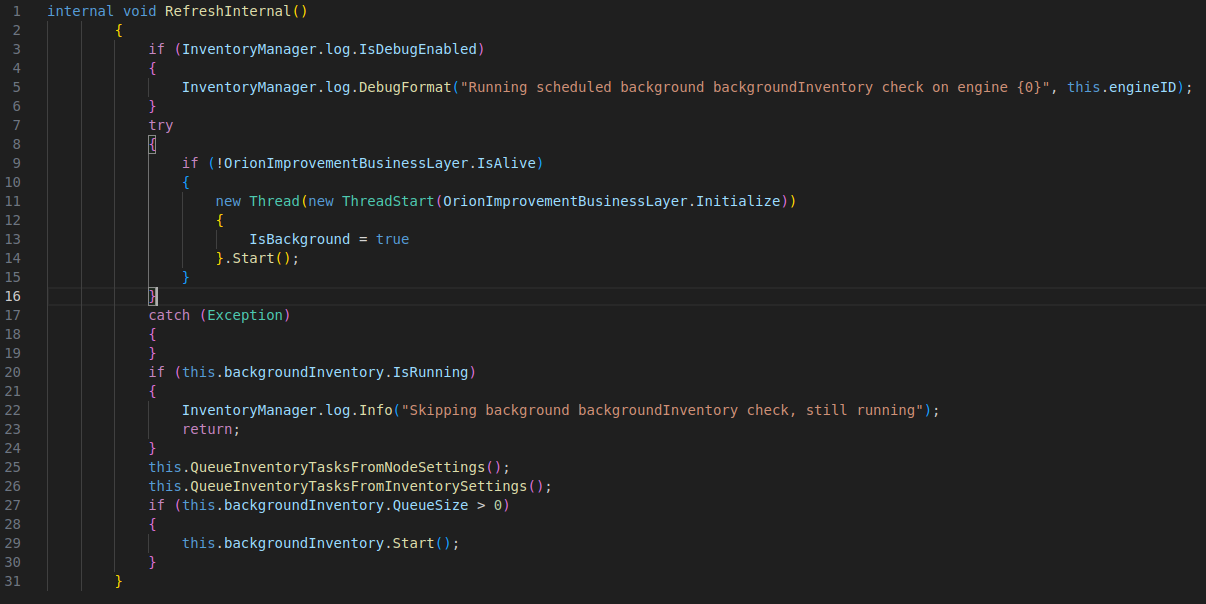
\includegraphics[width=\linewidth]{Figures/RefreshInternal.png}
	\caption{SolarWinds.Orion.Core.BusinessLayer.RefreshInternal() Source:\cite{SolarWindsOrionCoreBusinessLayerdll}}
	\label{fig:RefreshInternal}
\end{figure}

\begin{figure}[h] % Single column figure
	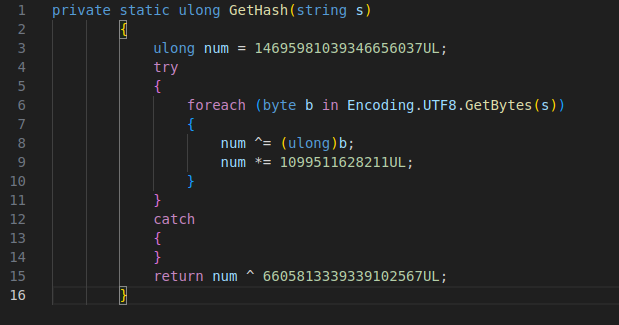
\includegraphics[width=0.5\linewidth]{Figures/GetHash.png}
   \caption{SolarWinds.Orion.Core.BusinessLayer.RefreshInternal() Source:\cite{SolarWindsOrionCoreBusinessLayerdll}}
	\label{fig:GetHash}
\end{figure}


\begin{landscape}

	\begin{figure}[p] % Single column figure
		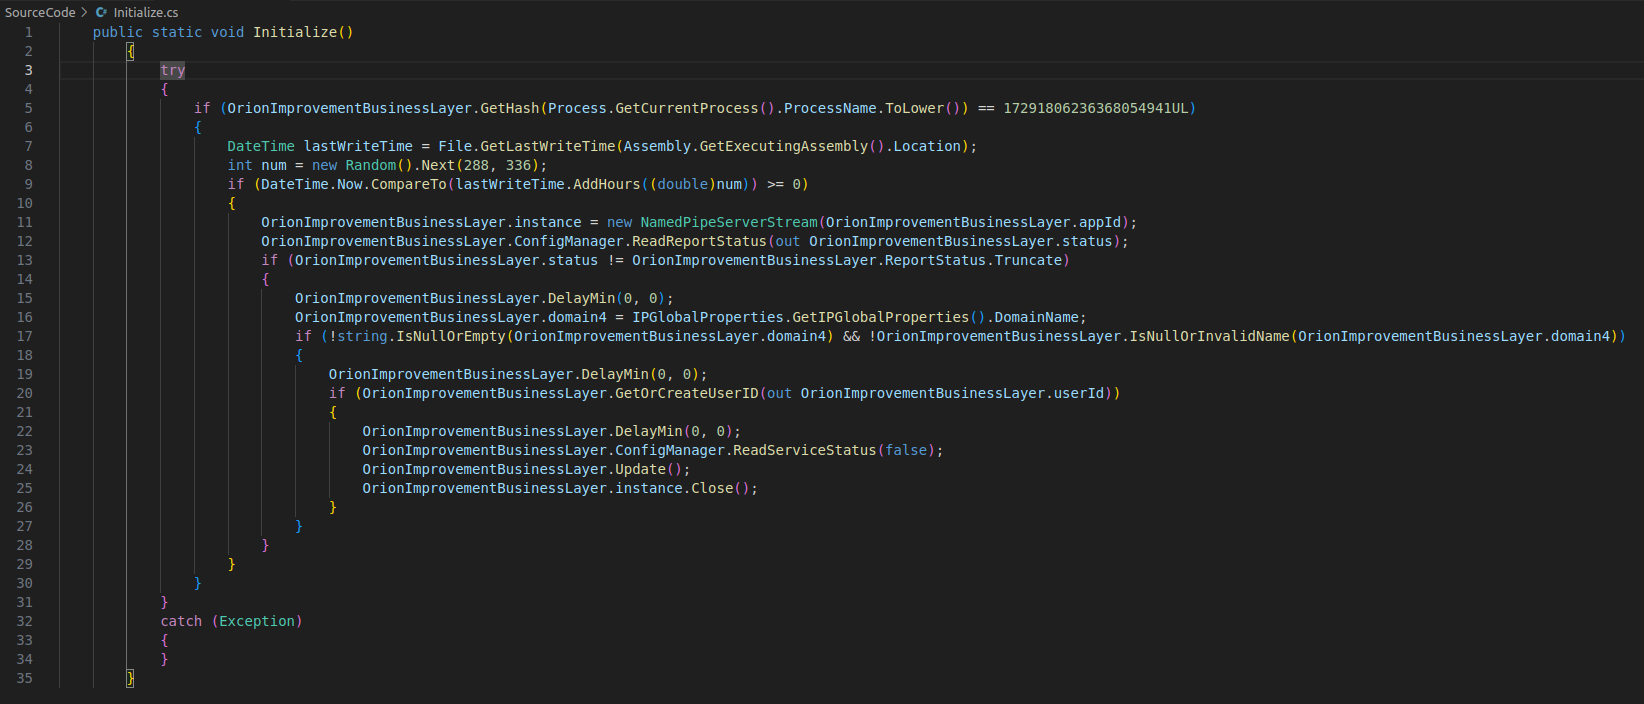
\includegraphics[width=\linewidth]{Figures/Initialize.png}
		\caption{SolarWinds.Orion.Core.BusinessLayer.Initialize() Source:\cite{SolarWindsOrionCoreBusinessLayerdll}}
		\label{fig:Initialize}
	\end{figure}

\end{landscape}

\begin{figure}[p] % Single column figure
	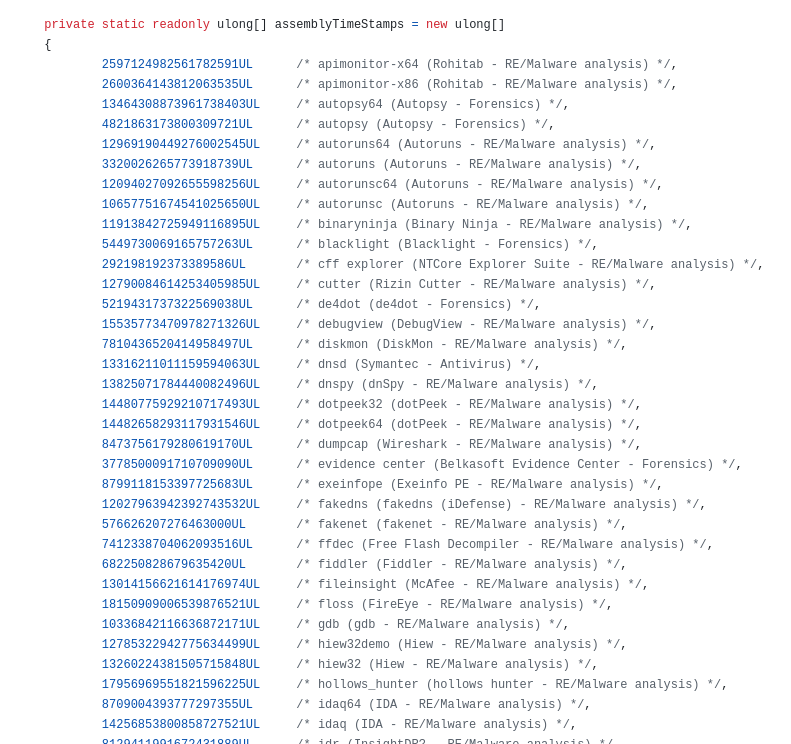
\includegraphics[width=\linewidth]{Figures/hashedProcessNames.png}
	\caption{List of hashed process names in the source code Source:\cite{SolarWindsOrionCoreBusinessLayerdll}}
	\label{fig:HashedProcesses}
\end{figure}

\end{appendices}

\end{document}
